\documentclass[11pt,a4paper]{report}
\usepackage[textwidth=37em,vmargin=30mm]{geometry}
\usepackage{calc,xunicode,amsmath,amssymb,paralist,enumitem,tabu,booktabs,datetime2,xeCJK,xeCJKfntef,listings}
\usepackage{tocloft,fancyhdr,tcolorbox,xcolor,graphicx,eso-pic,xltxtra,xelatexemoji}

\newcommand{\envyear}[0]{2025}
\newcommand{\envdatestr}[0]{2025-06-10}
\newcommand{\envfinaldir}[0]{webdb/2025/20250610/final}

\usepackage[hidelinks]{hyperref}
\hypersetup{
    colorlinks=false,
    pdfpagemode=FullScreen,
    pdftitle={Web Digest - \envdatestr}
}

\setlength{\cftbeforechapskip}{10pt}
\renewcommand{\cftchapfont}{\rmfamily\bfseries\large\raggedright}
\setlength{\cftbeforesecskip}{2pt}
\renewcommand{\cftsecfont}{\sffamily\small\raggedright}

\setdefaultleftmargin{2em}{2em}{1em}{1em}{1em}{1em}

\usepackage{xeCJK,xeCJKfntef}
\xeCJKsetup{PunctStyle=plain,RubberPunctSkip=false,CJKglue=\strut\hskip 0pt plus 0.1em minus 0.05em,CJKecglue=\strut\hskip 0.22em plus 0.2em}
\XeTeXlinebreaklocale "zh"
\XeTeXlinebreakskip = 0pt


\setmainfont{Brygada 1918}
\setromanfont{Brygada 1918}
\setsansfont{IBM Plex Sans}
\setmonofont{JetBrains Mono NL}
\setCJKmainfont{Noto Serif CJK SC}
\setCJKromanfont{Noto Serif CJK SC}
\setCJKsansfont{Noto Sans CJK SC}
\setCJKmonofont{Noto Sans CJK SC}

\setlength{\parindent}{0pt}
\setlength{\parskip}{8pt}
\linespread{1.15}

\lstset{
	basicstyle=\ttfamily\footnotesize,
	numbersep=5pt,
	backgroundcolor=\color{black!5},
	showspaces=false,
	showstringspaces=false,
	showtabs=false,
	tabsize=2,
	captionpos=b,
	breaklines=true,
	breakatwhitespace=true,
	breakautoindent=true,
	linewidth=\textwidth
}






\newcommand{\coverpic}[2]{
    % argv: itemurl, authorname
    Cover photo by #2~~(\href{#1}{#1})
}
\newcommand{\makeheader}[0]{
    \begin{titlepage}
        % \newgeometry{hmargin=15mm,tmargin=21mm,bmargin=12mm}
        \begin{center}
            
            \rmfamily\scshape
            \fontspec{BaskervilleF}
            \fontspec{Old Standard}
            \fontsize{59pt}{70pt}\selectfont
            WEB\hfill DIGEST
            
            \vfill
            % \vskip 30pt
            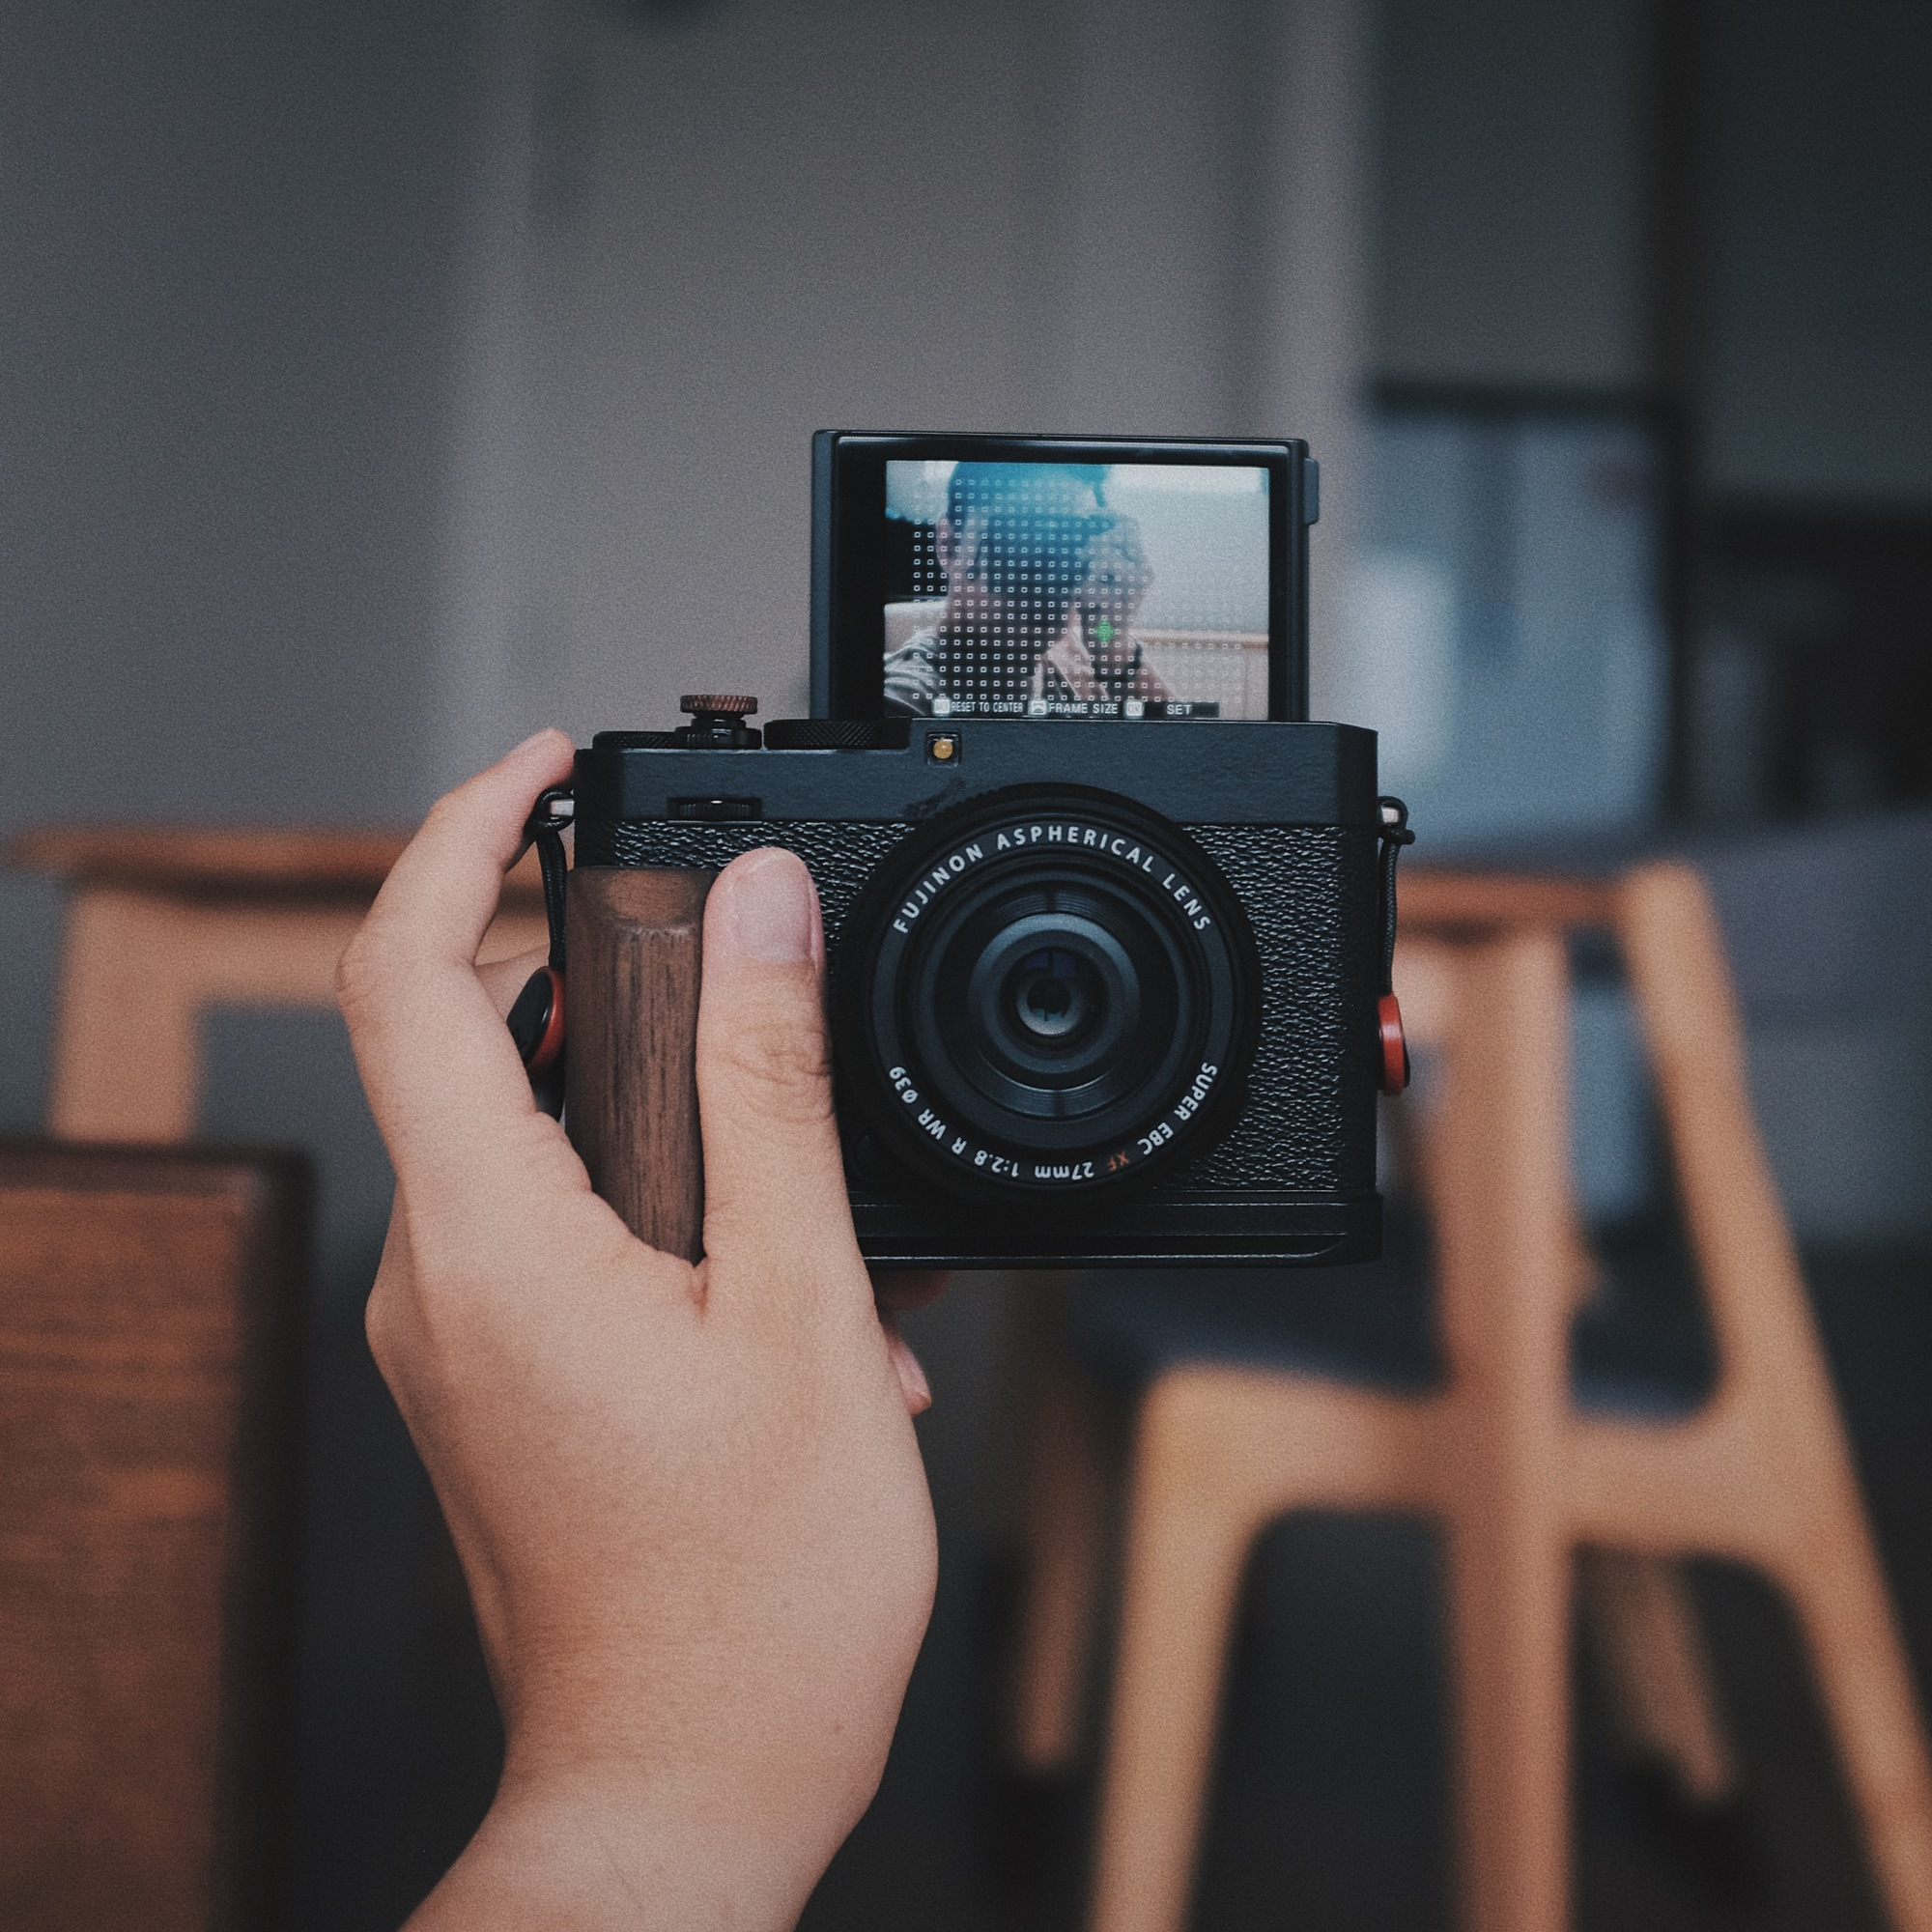
\includegraphics[width=\linewidth]{\envfinaldir/coverpic-prod.jpg}\par
            % \vskip 30pt
            \vfill

            \normalsize\rmfamily\scshape
            \copyright{} The Web Digest Project \hfill\large \envdatestr
        \end{center}
    \end{titlepage}
    % \restoregeometry
}
\newcommand{\simplehref}[1]{%
    \textcolor{blue!80!green}{\href{#1}{#1}}%
}
\renewcommand{\contentsname}{\center\Huge\sffamily\bfseries Contents\par\vskip 20pt}
\newcounter{ipartcounter}
\setcounter{ipartcounter}{0}
\newcommand{\ipart}[1]{
    % \vskip 20pt
    \clearpage
    \stepcounter{ipartcounter}
    \phantomsection
    \addcontentsline{toc}{chapter}{#1}
    % \begin{center}
    %     \Huge
    %     \sffamily\bfseries
    %     #1
    % \end{center}
    % \vskip 20pt plus 7pt
}
\newcounter{ichaptercounter}
\setcounter{ichaptercounter}{0}
\newcommand{\ichapter}[1]{
    % \vskip 20pt
    \clearpage
    \stepcounter{ichaptercounter}
    \phantomsection
    \addcontentsline{toc}{section}{\numberline{\arabic{ichaptercounter}}#1}
    \begin{center}
        \Huge
        \sffamily\bfseries
        #1
    \end{center}
    \vskip 20pt plus 7pt
}
\newcommand{\entrytitlefont}[1]{\subsection*{\raggedright\Large\sffamily\bfseries#1}}
\newcommand{\entryitemGeneric}[2]{
    % argv: title, url
    \parbox{\linewidth}{
        \entrytitlefont{#1}\par\vskip 5pt
        \footnotesize\ttfamily\mdseries
        \simplehref{#2}
    }\vskip 11pt plus 11pt minus 1pt
}
\newcommand{\entryitemGithub}[3]{
    % argv: title, url, desc
    \parbox{\linewidth}{
        \entrytitlefont{#1}\par\vskip 5pt
        \footnotesize\ttfamily\mdseries
        \simplehref{#2}\par\vskip 5pt
        \small\rmfamily\mdseries#3
    }\vskip 11pt plus 11pt minus 1pt
}
\newcommand{\entryitemAp}[3]{
    % argv: title, url, desc
    \parbox{\linewidth}{
        \entrytitlefont{#1}\par\vskip 5pt
        \footnotesize\ttfamily\mdseries
        \simplehref{#2}\par\vskip 5pt
        \small\rmfamily\mdseries#3
    }\vskip 11pt plus 11pt minus 1pt
}
\newcommand{\entryitemHackernews}[3]{
    % argv: title, hnurl, rawurl
    % \parbox{\linewidth}{
    %     \entrytitlefont{#1}\par\vskip 5pt
    %     \footnotesize\ttfamily\mdseries
    %     \simplehref{#3}\par
    %     \textcolor{black!50}{\href{#2}{#2}}
    % }\vskip 11pt plus 11pt minus 1pt
    \begin{minipage}{\linewidth}
            \entrytitlefont{#1}\par\vskip 5pt
            \footnotesize\ttfamily\mdseries
            \simplehref{#3}\par
            \textcolor{black!50}{\href{#2}{#2}}
    \end{minipage}\par\vskip 11pt plus 11pt minus 1pt
}







\begin{document}

\makeheader

\tableofcontents\clearpage




\ipart{Developers}
\ichapter{Hacker News}
\entryitemTwoLinks{RFK Jr. ousts entire CDC vaccine advisory committee}{https://news.ycombinator.com/item?id=44229778}{https://apnews.com/article/kennedy-cdc-acip-vaccines-3790c89f45b6314c5c7b686db0e3a8f9}

\entryitemTwoLinks{Kennedy guts CDC's vaccine panel of independent experts}{https://news.ycombinator.com/item?id=44229533}{https://www.nbcnews.com/health/health-news/kennedy-guts-acip-cdc-vaccine-panel-rcna211935}

\entryitemTwoLinks{Containerization is a Swift package for running Linux containers on macOS}{https://news.ycombinator.com/item?id=44229348}{https://github.com/apple/containerization}

\entryitemTwoLinks{A bit more on Twitter/X's new encrypted messaging}{https://news.ycombinator.com/item?id=44227689}{https://blog.cryptographyengineering.com/2025/06/09/a-bit-more-on-twitter-xs-new-encrypted-messaging/}

\entryitemTwoLinks{Apple announces Foundation Models and Containerization frameworks, etc}{https://news.ycombinator.com/item?id=44226978}{https://www.apple.com/newsroom/2025/06/apple-supercharges-its-tools-and-technologies-for-developers/}

\entryitemTwoLinks{Show HN: Munal OS: a graphical experimental OS with WASM sandboxing}{https://news.ycombinator.com/item?id=44226879}{https://github.com/Askannz/munal-os}

\entryitemTwoLinks{Apple introduces a universal design across platforms}{https://news.ycombinator.com/item?id=44226612}{https://www.apple.com/newsroom/2025/06/apple-introduces-a-delightful-and-elegant-new-software-design/}

\entryitemTwoLinks{Tell HN: Help restore the tax deduction for software dev in the US (Section 174)}{https://news.ycombinator.com/item?id=44226145}{https://news.ycombinator.com/item?id=44226145}

\entryitemTwoLinks{Show HN: Most users won't report bugs unless you make it stupidly easy}{https://news.ycombinator.com/item?id=44225352}{https://news.ycombinator.com/item?id=44225352}

\entryitemTwoLinks{Hokusai Moyo Gafu: an album of dyeing patterns}{https://news.ycombinator.com/item?id=44224992}{https://ndlsearch.ndl.go.jp/en/imagebank/theme/hokusaimoyo}

\entryitemTwoLinks{Doctors could hack the nervous system with ultrasound}{https://news.ycombinator.com/item?id=44224874}{https://spectrum.ieee.org/focused-ultrasound-stimulation-inflammation-diabetes}

\entryitemTwoLinks{Bruteforcing the phone number of any Google user}{https://news.ycombinator.com/item?id=44224684}{https://brutecat.com/articles/leaking-google-phones}

\entryitemTwoLinks{Defiant loyalists paid dearly for choosing wrong side in the American Revolution}{https://news.ycombinator.com/item?id=44223853}{https://www.smithsonianmag.com/history/meet-the-defiant-loyalists-who-paid-dearly-for-choosing-the-wrong-side-in-the-american-revolution-180986716/}

\entryitemTwoLinks{LLMs are cheap}{https://news.ycombinator.com/item?id=44223448}{https://www.snellman.net/blog/archive/2025-06-02-llms-are-cheap/}

\entryitemTwoLinks{Ex-FCC Chair Ajit Pai is now a wireless lobbyist}{https://news.ycombinator.com/item?id=44223283}{https://arstechnica.com/tech-policy/2025/06/ex-fcc-chair-ajit-pai-is-now-a-wireless-lobbyist-and-enemy-of-cable-companies/}

\entryitemTwoLinks{EU OS for the Public Sector}{https://news.ycombinator.com/item?id=44222896}{https://eu-os.eu/}

\entryitemTwoLinks{AI Angst}{https://news.ycombinator.com/item?id=44222885}{https://www.tbray.org/ongoing/When/202x/2025/06/06/My-AI-Angst}

\entryitemTwoLinks{Finding Shawn Mendes (2019)}{https://news.ycombinator.com/item?id=44222119}{https://ericneyman.wordpress.com/2019/11/26/finding-shawn-mendes/}

\entryitemTwoLinks{Forests offset warming more than thought: study}{https://news.ycombinator.com/item?id=44221489}{https://news.ucr.edu/articles/2025/05/29/does-planting-trees-really-help-cool-planet}

\entryitemTwoLinks{Kagi Reaches 50k Users}{https://news.ycombinator.com/item?id=44221450}{https://kagi.com/stats?stat=members}\ichapter{GitHub}
\entryitemWithDescription{\hskip 0pt{}jellyfin/jellyfin}{https://github.com/jellyfin/jellyfin}{The Free Software Media System - Server Backend \& API\\
Language: C\#\\
Stars: 40510\\
Forks: 3613}\ichapter{Dribbble}
\entryitemGeneric{\hskip 0pt{}Aquasan}{https://dribbble.com/shots/26100535-Aquasan}

\entryitemGeneric{\hskip 0pt{}Eagle}{https://dribbble.com/shots/26099428-Eagle}

\entryitemGeneric{\hskip 0pt{}Mnp Technologies - Logo Design}{https://dribbble.com/shots/26092034-Mnp-Technologies-Logo-Design}

\entryitemGeneric{\hskip 0pt{}Singular Logo Concept (Unused)}{https://dribbble.com/shots/26091755-Singular-Logo-Concept-Unused}

\entryitemGeneric{\hskip 0pt{}Cre8tera // Website}{https://dribbble.com/shots/26091009-Cre8tera-Website}

\entryitemGeneric{\hskip 0pt{}Cool Pool Logo Design - Letter C Monogram}{https://dribbble.com/shots/26091401-Cool-Pool-Logo-Design-Letter-C-Monogram}

\entryitemGeneric{\hskip 0pt{}Gorilla + Bar Chart Logo}{https://dribbble.com/shots/26092670-Gorilla-Bar-Chart-Logo}

\entryitemGeneric{\hskip 0pt{}zeero logo design}{https://dribbble.com/shots/26087342-zeero-logo-design}

\entryitemGeneric{\hskip 0pt{}Create email inbox composition}{https://dribbble.com/shots/26083118-Create-email-inbox-composition}

\entryitemGeneric{\hskip 0pt{}Shori Brand}{https://dribbble.com/shots/26088139-Shori-Brand}

\entryitemGeneric{\hskip 0pt{}Roaring Bear}{https://dribbble.com/shots/26087788-Roaring-Bear}

\entryitemGeneric{\hskip 0pt{}Eagle}{https://dribbble.com/shots/26085536-Eagle}

\entryitemGeneric{\hskip 0pt{}Hand-drawn illustration pack}{https://dribbble.com/shots/26084735-Hand-drawn-illustration-pack}

\entryitemGeneric{\hskip 0pt{}Dog Mascot Various Poses}{https://dribbble.com/shots/26087977-Dog-Mascot-Various-Poses}

\entryitemGeneric{\hskip 0pt{}Branding Concept for Europe}{https://dribbble.com/shots/26087652-Branding-Concept-for-Europe}

\entryitemGeneric{\hskip 0pt{}B2B Dashboard \& Web App UI UX Design for Carbon Solutions}{https://dribbble.com/shots/26076624-B2B-Dashboard-Web-App-UI-UX-Design-for-Carbon-Solutions}

\entryitemGeneric{\hskip 0pt{}Patriot Logo Design (Unused for Sale)}{https://dribbble.com/shots/26081047-Patriot-Logo-Design-Unused-for-Sale}

\entryitemGeneric{\hskip 0pt{}Heliopoint}{https://dribbble.com/shots/26081987-Heliopoint}

\entryitemGeneric{\hskip 0pt{}Apple}{https://dribbble.com/shots/26084067-Apple}

\entryitemGeneric{\hskip 0pt{}Illustration}{https://dribbble.com/shots/26083223-Illustration}

\entryitemGeneric{\hskip 0pt{}Europe Logo Animation}{https://dribbble.com/shots/26082596-Europe-Logo-Animation}

\entryitemGeneric{\hskip 0pt{}Arc Logo}{https://dribbble.com/shots/26083648-Arc-Logo}

\entryitemGeneric{\hskip 0pt{}Heyo Turns 2!}{https://dribbble.com/shots/26078572-Heyo-Turns-2}

\entryitemGeneric{\hskip 0pt{}Fox Brand Mascot}{https://dribbble.com/shots/26077954-Fox-Brand-Mascot}


\ipart{Developers~~~~(zh-Hans)}
\ichapter{Solidot}
\entryitemGeneric{\hskip 0pt{}安全阻碍了企业拥抱 AI}{https://www.solidot.org/story?sid=81506}

\entryitemGeneric{\hskip 0pt{}谷歌CEO皮查伊:为什么说AI意义将超越火与电?}{https://www.solidot.org/story?sid=81505}

\entryitemGeneric{\hskip 0pt{}Google 塑造的 Web 也许将被重塑}{https://www.solidot.org/story?sid=81504}

\entryitemGeneric{\hskip 0pt{}微软第一方游戏进入 80 美元时代}{https://www.solidot.org/story?sid=81503}

\entryitemGeneric{\hskip 0pt{}Linux 6.16-rc1 释出}{https://www.solidot.org/story?sid=81502}

\entryitemGeneric{\hskip 0pt{}微软和华硕合作推出 Xbox 掌机 ROG Xbox Ally}{https://www.solidot.org/story?sid=81501}

\entryitemGeneric{\hskip 0pt{}Kagi 用户数突破五万}{https://www.solidot.org/story?sid=81500}

\entryitemGeneric{\hskip 0pt{}欧盟新规定强制要求为智能手机和平板提供五年操作系统更新}{https://www.solidot.org/story?sid=81499}

\entryitemGeneric{\hskip 0pt{}/e/OS 3.0 释出}{https://www.solidot.org/story?sid=81498}

\entryitemGeneric{\hskip 0pt{}Android 应用面临越来越多的不兼容问题}{https://www.solidot.org/story?sid=81497}

\entryitemGeneric{\hskip 0pt{}越南废除二孩政策}{https://www.solidot.org/story?sid=81496}

\entryitemGeneric{\hskip 0pt{}天文学家发现中等质量黑洞的新证据}{https://www.solidot.org/story?sid=81495}

\entryitemGeneric{\hskip 0pt{}英国考虑推出数字 ID 卡}{https://www.solidot.org/story?sid=81494}

\entryitemGeneric{\hskip 0pt{}就读美国大学的中国留学生人数持续下降}{https://www.solidot.org/story?sid=81493}

\entryitemGeneric{\hskip 0pt{}YouTube 以有害内容下架主播的自我托管视频内容的教程}{https://www.solidot.org/story?sid=81492}\ichapter{V2EX}
\entryitemGeneric{\hskip 0pt{}[推广] 搬瓦工荷兰 EUNL1 三网优化机 新出江湖}{https://www.v2ex.com/t/1137499}

\entryitemGeneric{\hskip 0pt{}[macOS] macOS Tahoe is the final major version for Intel-based Macs}{https://www.v2ex.com/t/1137498}

\entryitemGeneric{\hskip 0pt{}[分享创造] 分享一个 V2EX 更好的评论油猴脚本,支持自定义表情和快速上传图片}{https://www.v2ex.com/t/1137496}

\entryitemGeneric{\hskip 0pt{}[问与答] 杭州西湖区如何骑摩托车避免被罚?}{https://www.v2ex.com/t/1137495}

\entryitemGeneric{\hskip 0pt{}[New York] 有纽约的大咖需要 UI 设计界面服务?}{https://www.v2ex.com/t/1137494}

\entryitemGeneric{\hskip 0pt{}[问与答] 组件库实战-基建思路}{https://www.v2ex.com/t/1137493}

\entryitemGeneric{\hskip 0pt{}[问与答] 求助:刚买的云服务器无法 ssh 连接}{https://www.v2ex.com/t/1137491}

\entryitemGeneric{\hskip 0pt{}[问与答] 看了惠威 os10 和漫步者 mr5bt,同样天猫 799 该怎么选}{https://www.v2ex.com/t/1137489}

\entryitemGeneric{\hskip 0pt{}[问与答] 我看到了一场霸凌,我决定做点什么}{https://www.v2ex.com/t/1137488}

\entryitemGeneric{\hskip 0pt{}[分享发现] 原来 wechat 在去年底修订的隐私策略就删除了``不显示个性化广告''条目}{https://www.v2ex.com/t/1137487}

\entryitemGeneric{\hskip 0pt{}[分享创造] 新模型 Flux Kontext, API 价格比官网 8 倍}{https://www.v2ex.com/t/1137486}

\entryitemGeneric{\hskip 0pt{}[问与答] 求问我应该买 MacBook Air 还是买 pro?}{https://www.v2ex.com/t/1137485}

\entryitemGeneric{\hskip 0pt{}[Android] 为什么淘宝京东美团这类软件在后台切换回来时会很卡?}{https://www.v2ex.com/t/1137484}

\entryitemGeneric{\hskip 0pt{}[全球工单系统] 疑似 CloudFlare CDN 解析被墙 ip}{https://www.v2ex.com/t/1137482}

\entryitemGeneric{\hskip 0pt{}[程序员] AI 学习}{https://www.v2ex.com/t/1137480}

\entryitemGeneric{\hskip 0pt{}[问与答] Java 开发,目前快 3 年经验,怎么才能提升自己的技术能力, V 友们有什么学习的经验吗,求指点}{https://www.v2ex.com/t/1137478}

\entryitemGeneric{\hskip 0pt{}[Linux] Linux 桌面, 小白用户不要硬上}{https://www.v2ex.com/t/1137477}

\entryitemGeneric{\hskip 0pt{}[Windows] 我最近 windows 10 某次更新后,輸入法就自動變成繁體了}{https://www.v2ex.com/t/1137476}

\entryitemGeneric{\hskip 0pt{}[北京] [求租] 京牌新能源指标, 5000/年}{https://www.v2ex.com/t/1137475}

\entryitemGeneric{\hskip 0pt{}[分享发现] 关于购买 NS2,分享一点自己的心得}{https://www.v2ex.com/t/1137474}

\entryitemGeneric{\hskip 0pt{}[Linux] 放弃 Linux 桌面的多屏用户,放弃前没考虑过怎么优雅的和 Windows 同时使用吗?}{https://www.v2ex.com/t/1137473}

\entryitemGeneric{\hskip 0pt{}[问与答] 现在还有什么稳妥的海外保号卡}{https://www.v2ex.com/t/1137472}

\entryitemGeneric{\hskip 0pt{}[分享创造] 餐饮会是下一个被 ai 冲击的行业吗}{https://www.v2ex.com/t/1137471}

\entryitemGeneric{\hskip 0pt{}[广州] 海珠区客村附近粤菜馆推荐}{https://www.v2ex.com/t/1137470}

\entryitemGeneric{\hskip 0pt{}[设计] draw.io 的创新用途}{https://www.v2ex.com/t/1137469}

\entryitemGeneric{\hskip 0pt{}[程序员] 2025 年移动开发推荐用哪些框架啊}{https://www.v2ex.com/t/1137468}

\entryitemGeneric{\hskip 0pt{}[编程] cursor 还能用了吗?}{https://www.v2ex.com/t/1137467}

\entryitemGeneric{\hskip 0pt{}[WWDC] [WWDC25] 来了!再次开放直播交流群,本次直播我们一起讨论 OS26 在视觉和交互上的创新}{https://www.v2ex.com/t/1137466}

\entryitemGeneric{\hskip 0pt{}[问与答] 2025 年安卓上最好用的自动化模拟点击的工具推荐?}{https://www.v2ex.com/t/1137465}

\entryitemGeneric{\hskip 0pt{}[云计算] 自动修改 Grub,给 Linux 安装救援模式的脚本,特别适用于云服务器}{https://www.v2ex.com/t/1137461}

\entryitemGeneric{\hskip 0pt{}[程序员] 单片机如果存储空间紧张,就避免用 printf 类的函数}{https://www.v2ex.com/t/1137456}

\entryitemGeneric{\hskip 0pt{}[VPS] 为什么在 vps 运营商的网站看不到高性价比的套餐?}{https://www.v2ex.com/t/1137454}

\entryitemGeneric{\hskip 0pt{}[数据库] 关于数据库索引的一个问题:有复合索引建立于列 a,b,c。那么 where a=1 and b like b\% and c=3 命中此索引吗? where a=1 and b > 2 and c=3 命中此索引吗?}{https://www.v2ex.com/t/1137452}

\entryitemGeneric{\hskip 0pt{}[宽带症候群] 两个没有公网 IP 的海外内网间如何组网並分流 Netflix}{https://www.v2ex.com/t/1137451}

\entryitemGeneric{\hskip 0pt{}[上海] 刚才吃饭 ,一个许久不见的情况}{https://www.v2ex.com/t/1137450}

\entryitemGeneric{\hskip 0pt{}[Telegram] 电报代付平台靠谱吗?}{https://www.v2ex.com/t/1137448}

\entryitemGeneric{\hskip 0pt{}[投资] 活钱 05| 6 大好处+3 张表!科学记账全攻略}{https://www.v2ex.com/t/1137447}

\entryitemGeneric{\hskip 0pt{}[分享创造] 简单做了一个 prompt 提示词生成工具}{https://www.v2ex.com/t/1137446}

\entryitemGeneric{\hskip 0pt{}[汽车] 车险哪个渠道买便宜点?}{https://www.v2ex.com/t/1137444}

\entryitemGeneric{\hskip 0pt{}[生活] 联通给我打电话让我把移动宽带换掉}{https://www.v2ex.com/t/1137443}

\entryitemGeneric{\hskip 0pt{}[酷工作] [广州] 招聘 AI 算法工程师\&Electron 工程师(AI 方向) [高薪、多岗位、急招]}{https://www.v2ex.com/t/1137442}

\entryitemGeneric{\hskip 0pt{}[宽带症候群] 两个局域网如何互通}{https://www.v2ex.com/t/1137441}

\entryitemGeneric{\hskip 0pt{}[问与答] 求教:手机/笔记本电脑/路由器/便携屏之类的只有只有正负极输入的小功率设备,带地线的电源适配器有作用吗?}{https://www.v2ex.com/t/1137440}

\entryitemGeneric{\hskip 0pt{}[分享创造] 🚀 Velokit:基于 Next.js 15 + Supabase 的现代全栈模板,开箱即用}{https://www.v2ex.com/t/1137438}

\entryitemGeneric{\hskip 0pt{}[程序员] 恭喜 KDE,又一个操作系统 (FreeBSD) 打算把 KDE 设为首选桌面环境}{https://www.v2ex.com/t/1137436}

\entryitemGeneric{\hskip 0pt{}[Node.js] 不用继承就能给类加事件系统?这波原型链操作我给满分}{https://www.v2ex.com/t/1137432}

\entryitemGeneric{\hskip 0pt{}[问与答] 求一款安卓密码本,感觉 keepass 不好用}{https://www.v2ex.com/t/1137431}

\entryitemGeneric{\hskip 0pt{}[生活] 感觉自己被监控了,想不通问题出在哪里}{https://www.v2ex.com/t/1137430}

\entryitemGeneric{\hskip 0pt{}[DNS] 有没有可以检测返回结果可用性的工具}{https://www.v2ex.com/t/1137427}

\entryitemGeneric{\hskip 0pt{}[云计算] 大家说阿里云是个草台班子,真不冤}{https://www.v2ex.com/t/1137426}


\ipart{Generic News}
\ichapter{联合早报}
\entryitemWithDescription{中美伦敦启动经贸会谈 特朗普政府料急切求成以推他国谈判}{https://www.zaobao.com/news/china/story20250610-6643588}{中美谈判代表在伦敦当地时间星期一(6月9日)启动经贸会谈,这是中美贸易战爆发以来第二轮正式磋商。白宫官员称,美国在中国放宽稀土出口限制的前提下,愿意考虑取消部分对华出口限制。 受访学者指出,此次伦敦会谈是中美元首通话后直接促成,显示双方对磋商高度重视,预料代表团不愿空手而归。不过,华盛顿在当前阶段更迫切希望取得成果,以推动与其他国家的谈判进展……}

\entryitemWithDescription{中国5月出口放缓价格指数双降}{https://www.zaobao.com/news/china/story20250609-6643626}{受中美关税战影响,中国5月出口增速继续放缓,尤其是对美出口进一步恶化;中国国内居民消费价格和生产价格指数也双双下跌。 受访学者和分析师指出,最新数据显示中国居民消费疲软,企业陷入价格战,通缩压力加剧。但外贸展现出的韧性和核心通胀率上升,为经济潜在转机带来一些希望……}

\entryitemWithDescription{海峡论坛6月中旬在福建举办 台湾禁中央机关人员参会}{https://www.zaobao.com/news/china/story20250609-6642649}{(北京/台北综合讯)中国大陆国台办星期一(6月9日)宣布,第十七届海峡论坛将于6月中旬在福建举办。台湾陆委会此前强调,禁止中央机关人员以任何形式参与论坛。 据国台办官网,国台办发言人朱凤莲在发布会上说,本届海峡论坛集中活动为期一周,主会场设在福建厦门,福建有关设区市和平潭综合实验区也将举办相关活动。其中,论坛大会将在6月15日上午举办……}

\entryitemWithDescription{大陆国防部喊话民进党:美制武器救不了自己的命}{https://www.zaobao.com/news/china/story20250609-6639011}{(北京综合讯)针对美国据报计划扩大对台军售规模,中国大陆国防部告诫台湾执政的民进党``美制武器救不了自己的命''。 据央视新闻报道,大陆国防部新闻局副局长、新闻发言人蒋斌星期一(6月9日)在例行记者会上回应美国对台军售问题时说,这是由美国和台独势力主导、侵犯大陆核心利益、妄图改变台海现状、推高台海紧张局势的又一起实证。大陆对此强烈不满、坚决反对……}

\entryitemWithDescription{日本通报辽宁舰队驶入西南经济水域}{https://www.zaobao.com/news/china/story20250609-6639314}{(东京/北京综合讯)日本军方星期天(6月8日)首次通报解放军辽宁舰编队驶入日本西南经济水域,同时表明中国海军可能深入太平洋,并首次被发现在第二岛链以东活动。针对中国海军活动范围扩大,日本内阁秘书长林芳正星期一(9日)表示已向北京提出交涉。 中国外交部发言人林剑星期一则在例行记者会上回应称,中国军舰在有关海域活动完全符合国际法和国际惯例;中国一贯奉行防御性国防政策,希望日本客观理性看待……}

\entryitemWithDescription{李家超:香港将维持港元与美元的联系汇率制}{https://www.zaobao.com/news/china/story20250609-6639789}{(香港讯)香港特区行政长官李家超说,尽管地缘政治紧张局势不断升级,一些人呼吁将港元与人民币挂钩,但香港将维持港元与美元的联系汇率制。 香港《南华早报》星期一(6月9日)刊登对李家超的专访。李家超说,联系汇率制一直面临压力,尤其在不确定的时期;但事实证明,``香港与美元的联系汇率制,是香港经济成功的根本因素之一''……}

\entryitemWithDescription{美学者:大陆若以导弹攻击台湾商港 即可达成封锁目的}{https://www.zaobao.com/news/china/story20250609-6638248}{美国军方近期多次警告北京对台动武的可能性急速上升,曾任美国国防部资深供应链问题专家的学者格尔茨(Eugene Gholz)指出,中国大陆只要运用导弹精准打击台湾商用港口,就能达成封锁台湾的目的。 过去一个月,美国两度公开预警中国大陆攻台风险迫在眉睫。首先是美国媒体5月中旬传出印太司令帕帕罗在夏威夷跟印太20多个盟国参与的活动中提到,中国近年在台海周边的军事行动已是战争登场前的排练,并非单纯演习……}

\entryitemWithDescription{中国将推广普及分娩镇痛服务}{https://www.zaobao.com/news/china/story20250609-6636875}{(北京/香港综合讯)中国政府将推动全国三级医院在今年底之前提供分娩镇痛服务,通过改善分娩体验,鼓励女性生育。 中国国家卫生健康委员会上星期四(6月5日)在官网发布《关于全面推进分娩镇痛工作的通知》,提出推动综合医院、妇产专科医院、妇幼保健机构等医疗机构广泛开展分娩镇痛服务……}

\entryitemWithDescription{波音时隔两个月恢复交付新飞机给中国飞机}{https://www.zaobao.com/news/china/story20250609-6637238}{(首尔/华盛顿综合讯)美国波音公司一架全新的737 MAX型客机,星期一(6月9日)在中国降落。这是时隔两个月波音再次对华交付飞机,显示尽管中美仍存在关税僵局,但双边贸易往来正逐步恢复。 综合路透社与彭博社报道,飞行跟踪数据显示,当地时间上周五(6日)上午10时,一架涂有厦门航空标志的波音 737 MAX客机从西雅图起飞,首站飞往夏威夷,星期一降落在上海附近的波音舟山完工与交付中心……}

\entryitemWithDescription{沈泽玮:中美进入深水区近战肉搏}{https://www.zaobao.com/news/china/story20250609-6626426}{中美元首通电话打破僵局后,两国新一轮谈判将于6月9日在英国伦敦登场。 中国外交部称它为``中美经贸磋商机制首次会议''。换句话说,双方5月初在瑞士日内瓦谈判建立起的经贸磋商机制,将迎来第一次会议。 从这个角度看,日内瓦谈判只是热身,休战90天只为缓冲,真正的深水区近战肉搏战将自伦敦谈判开打。全世界都等着看中美怎么谈、谈出什么来……}

\entryitemWithDescription{中美伦敦会谈前夕 中国称已批准一定数量的稀土出口许可申请}{https://www.zaobao.com/news/china/story20250608-6625081}{(北京综合讯)中国官方称已批准一定数量的稀土出口许可申请,在中美贸易会谈前夕,此举或有助于缓解两国之间的紧张局势。 中国商务部新闻发言人星期六(6月7日)晚在官网以答记者问的形式说,稀土相关物项具有军民两用属性,对其实施出口管制符合国际通行做法。中国依法对稀土相关物项实施出口管制,目的是更好维护国家安全和利益,履行防扩散等国际义务,体现了坚持维护世界和平与地区稳定的一贯立场……}

\entryitemWithDescription{监督机制欠缺 中国互联网企业贪腐案数量增加}{https://www.zaobao.com/news/china/story20250608-6468952}{中国官方针对互联网行业的反腐行动这些年来持续推进,官方数据显示,相关贪腐案件近年增加,且呈现人员年轻化、``小官巨贪''等特点。 受访学者指出,中国对于企业贪腐,尚未建立完善的社会治理机制,加上``流量为王''的时代给予互联网平台巨大的``平台软权力'',形成腐败温床。 北京市海淀区法院5月15日发布白皮书,通报海淀区过去五年审理的互联网企业贪腐案件概况,并分析这类犯罪背后的成因……}

\entryitemWithDescription{港媒:章立凡今年3月病逝}{https://www.zaobao.com/news/china/story20250608-6621755}{(香港讯)中国历史学者章立凡因病去世,享年74岁。 香港《明报》星期天(6月8日)报道上述消息,没有具体说明病因。报道引述知情者说,章立凡曾中风,今年3月去世,他的家人受到非常大的压力,因此他的死讯及丧事都处理得非常保密。报道没有说明章立凡的家人为何受到非常大的压力。 知情者还说,章立凡的骨灰星期六(7日)下葬在北京怀柔的九公山陵园……}

\entryitemWithDescription{台湾举行海安演习 应对大陆灰色地带威胁}{https://www.zaobao.com/news/china/story20250608-6625660}{(高雄综合讯)台湾军方与海巡署举行两年一度的海域安全军事演习,演练联合作战能力,应对来自中国大陆日益加剧的灰色地带威胁。 综合路透社、自由时报、风传媒等报道,台湾海洋委员会海巡署与国防部于星期天(6月8日)海洋日在高雄港举行``海安12号演习'',实兵操演海上拦截围捕、空中垂降救援,以及舰艇海空分列式三大项目……}

\entryitemWithDescription{李家超:香港不会向美国实施报复性关税}{https://www.zaobao.com/news/china/story20250608-6620899}{(香港综合讯)香港特区行政长官李家超承诺,即使中美地缘政治紧张局势进一步升级,香港也不会向美国征收报复性关税,以免破坏自身``成功基因''并危及自由港地位。 香港《南华早报》星期天(6月8日)刊登对李家超的专访。这名上任即将三年的特首说,香港的成功因素在于开放性,而香港作为贸易枢纽的地位得益于零关税和自由港政策,``你不会摧毁自己的成功基因''……}

\entryitemWithDescription{中国官方智库:南中国海周边国家要自己掌握解决问题钥匙}{https://www.zaobao.com/news/china/story20250608-6620837}{(北京综合讯)中国官方智库发布报告称,地区国家要把解决南中国海问题的钥匙掌握在自己手中,反对域外势力插手干涉。 据新华社报道,在第17个世界海洋日到来之际,新华社国家高端智库星期天(6月8日)发布中英文报告《中国将南海打造成和平、友谊、合作之海的实践》。 报告说,南中国海稳,则地区国家受益;南中国海乱,则地区国家遭殃;南中国海地区和平稳定是包括中国在内地区国家的共同愿望,符合各国利益……}

\entryitemWithDescription{中国特稿:晶片围困华 稀土将军美}{https://www.zaobao.com/news/china/story20250608-6581514}{``中东有石油,中国有稀土。'' 据中国媒体报道,这是已故中国改革开放总设计师邓小平在1992年说过的话。 邓小平或许没料到,33年后预言成真,稀土成了中国与美国地缘政治博弈的王牌……}

\entryitemWithDescription{美中6月9日伦敦会谈料聚焦稀土科技关税 学者:有望取得实质进展}{https://www.zaobao.com/news/china/story20250607-6605709}{美中领导人通话不到两天,美国总统特朗普星期五(6月6日)率先宣布,美方经贸官员将于星期一(6月9日)在伦敦与中方代表举行会谈。他也称,北京已同意恢复向美国供应稀土。 中国外交部发言人星期六(6月7日)晚随后证实,称中国国务院副总理何立峰将于6月8日至13日访问英国,其间,将与美方举行中美经贸磋商机制首次会议。 受访学者预料,中美在伦敦会谈将聚焦稀土、科技与关税等议题……}

\entryitemWithDescription{领导人峰会在即 中欧就电动车稀土等贸易问题取得进展}{https://www.zaobao.com/news/china/story20250607-6610128}{中欧领导人峰会在即,持续困扰双边关系的诸多贸易问题正取得进展,双方为中国产电动车制定最低价格的谈判进入最后阶段,北京也表态愿放宽对欧稀土出口,并将于7月5日前对欧盟白兰地反倾销案作出最终裁定……}

\entryitemWithDescription{民进党:最多可罢免10席以上国民党立委}{https://www.zaobao.com/news/china/story20250607-6606110}{(台北综合讯)台湾将在7月至8月启动罢免投票,执政的民进党内部评估认为,虽有多名党籍立委被连署提案罢免,但成功罢免的可能性不高;相较之下,国民党则可能有超过10席立委面临被罢免成功的风险。 综合《联合报》《上报》等报道,民进党人士分析,国民党原本认为原住民族选区``蓝大于绿'',因此率先对该选区的民进党立委陈莹与伍丽华发起罢免,未料两案第二阶段连署相继失败,重挫士气……}

\entryitemWithDescription{吉利董事长:汽车工业存在``严重的产能过剩''}{https://www.zaobao.com/news/china/story20250607-6609477}{(北京路透电)吉利控股集团董事长李书福说,当今世界的汽车工业存在``严重的产能过剩'',该公司已决定不再建设新的汽车生产工厂或扩大现有工厂的产能。 李书福星期六(6月7日)以视频方式参加在重庆举行的``中国汽车重庆论坛'',并发表上述讲话。 他说,吉利不搞重复建设,而要充分利用全球过剩的产能,尽最大可能地展开务实合作、资源重组……}

\entryitemWithDescription{台籍教师持中国大陆定居证遭废台湾身份 批陆委会非法滥权}{https://www.zaobao.com/news/china/story20250607-6606366}{(台北综合讯)在福建任教的台籍教师张立齐因持有中国大陆定居证被废止台湾身份,他随后批评台湾政府的大陆委员会``非法滥权迫害'',陆委会则回应称``少数人不要心存侥幸,挑战政府执法决心''。 综合《自由时报》《中国时报》报道,在福建华侨大学任教的张立齐,去年响应中国大陆融合发展政策,成为福建首名领取``台湾居民定居证''的台湾人……}






\clearpage
\leavevmode\vfill
\footnotesize

Copyright \copyright{} 2023-2025 Neruthes and other contributors.

This document is published with CC BY-NC-ND 4.0 license.

The entries listed in this newsletter may be copyrighted by their respective creators.

This newsletter is generated by the Web Digest project.

The newsletters are also delivered via Telegram channel \CJKunderline{\href{https://t.me/webdigestchannel}{https://t.me/webdigestchannel}}.\\
RSS feed is available at \CJKunderline{\href{https://webdigest.pages.dev/rss.xml}{https://webdigest.pages.dev/rss.xml}}.

This newsletter is available in PDF at
\CJKunderline{\href{https://webdigest.pages.dev/}{https://webdigest.pages.dev/}}.

The source code being used to generate this newsletter is available at\\
\CJKunderline{\href{https://github.com/neruthes/webdigest}{https://github.com/neruthes/webdigest}}.

This newsletter is also available in
\CJKunderline{\href{http://webdigest.pages.dev/readhtml/\envyear/WebDigest-20250610.html}{HTML}} and
\CJKunderline{\href{https://github.com/neruthes/webdigest/blob/master/markdown/\envyear/WebDigest-20250610.md}{Markdown}}.


\coverpic{https://unsplash.com/photos/a-blurry-photo-of-a-plant-on-a-wall-iMgi62f5MsE}{Kasia Sikorska}


\end{document}
